\subsection{Mineração de Dados}

O termo mineração de dados, de acordo com \citeAuthorPageYear{jmj} poderia ter sido chamado de mineração de conhecimentos dos dados, já que minerar é um processo para encontrar pequenas quantidades de preciosidades de uma grande quantidade de material bruto. 

Outros dizem que mineração de dados é um sinônimo de KDD (\textit{knowledge discovery from data}), descobrimento de conhecimento a partir de dados. A mineração também é vista como um passo essencial no processo de descoberta de conhecimento, como mostra a figura \ref{kdd}. 


\begin{figure}[H]
\centering
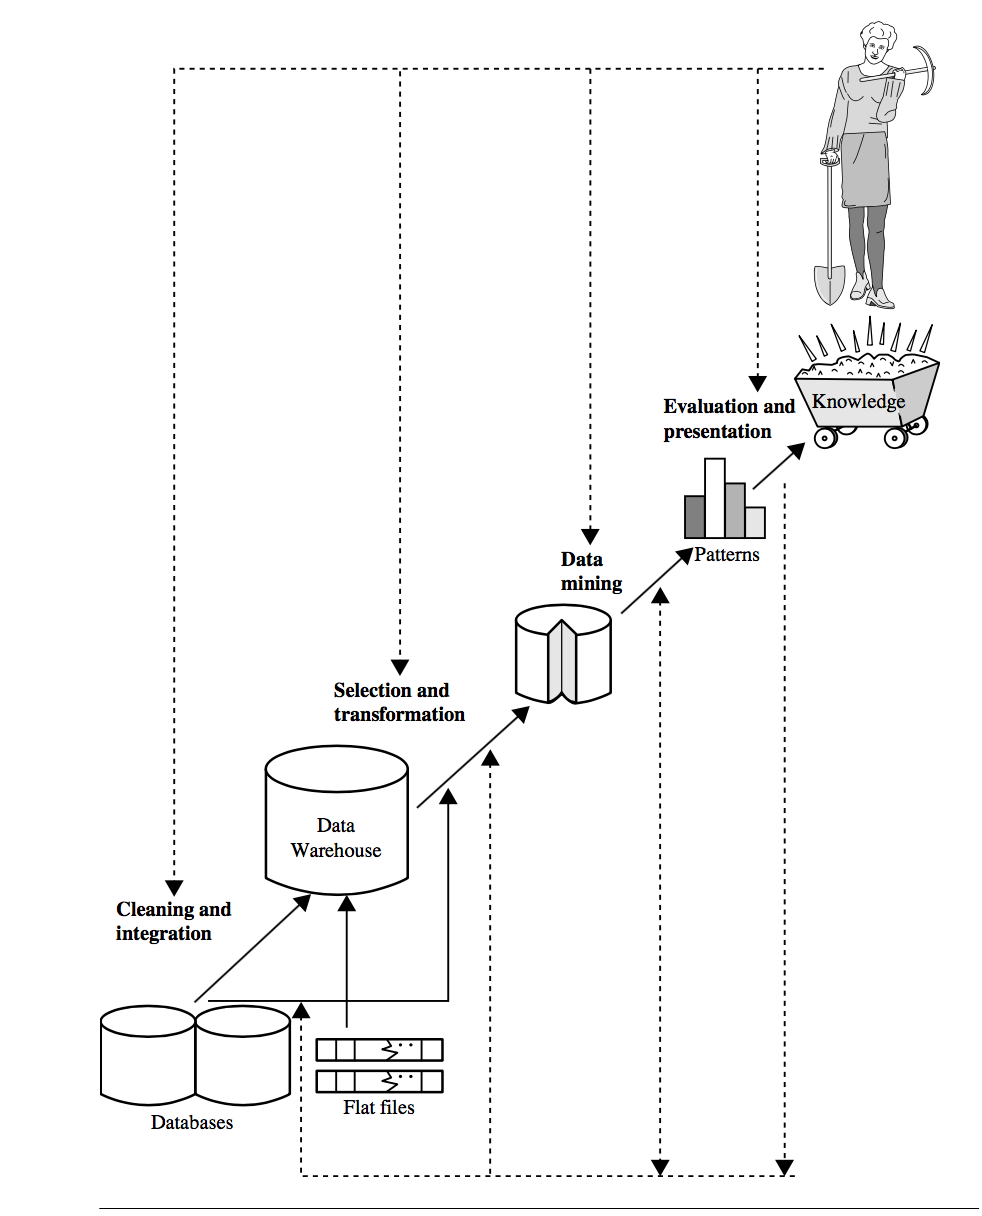
\includegraphics[height=9cm, width=9cm]{imagens/kdd.png}
\caption{Mineração de dados como um processo de descoberta de conhecimento \citep{jmj}}
\label{kdd}
\end{figure}

\citeAuthorPageYear{advancedDM} afirmam que massas de dados gerados de caixas registradoras, de bases de dados específicas, etc são exploradas, analisadas, reduzidas e reusadas. Ainda dizem que pesquisas são feitas através de diversos modelos para prever vendas, resposta de mercado, lucro, etc

Já \citeAuthorPageYear{jmj} afirmam que a mineração de dados tem diversas funcionalidades, como caracterização (sumarização das características gerais de uma classe alvo de dados) e discriminação (comparação das características gerais de uma classe alvo com as características de uma ou mais classes diferentes). 

Também é usada para encontrar padrões que aparecem frequentemente nos dados. Existem alguns tipos de padrões, como \textit{frequent itemset}, itens que geralmente aparecem juntos em um conjunto de dados transacionais, \textit{frequent subsequence} ou \textit{sequencial pattern}, que, por exemplo, é o padrão de um cliente que compra primeiro um \textit{notebook}, seguido de uma câmera digital e então um cartão de memória, de acordo com \citeAuthorPageYear{jmj}. Por último, tem as \textit{frequent substructures}, que são formas estruturadas que aparecem frequentemente, como grafos e árvores, que podem conter \textit{itemsets} e \textit{subsequences}.

Algoritmos de classificação, regressão, etc são usados para análises preditivas, tentando prever dados categóricos ou discretos. A classificação, segundo \citeAuthorPageYear{jmj}, é o processo de encontrar um modelo que melhor expressa uma classe. Esse modelo é derivado da análise de um conjunto de treinamento. Os modelos são representados usando árvores de decisão, fórmulas matemáticas, redes neurais etc.

Já a regressão, o uso mais comum é para tentar prever valores numéricos contínuos, com algoritmos como regressão linear, regressão LASSO etc.

De acordo com \citeAuthorPageYear{jmj}, também existem os algoritmos de clusterização, que, diferentemente da classificação e regressão, analisam os dados sem consultar as suas classes. Em alguns casos, os dados até vem sem classe. A clusterização é usada para encontrar classes para os grupos de dados. Os \textit{clusters} são formados de uma forma que os objetos dentro deles tenham uma grande similaridade ao se compararem uns com os outros, mas se diferenciam dos objetos em outros \textit{clusters}.
